\documentclass[10pt]{article}
\usepackage[a4paper,margin=13mm]{geometry}
\usepackage{amsmath,amssymb}
\usepackage{xcolor,tikz,fontspec}
\usetikzlibrary{arrows.meta,positioning,calc,fit,backgrounds,decorations.pathreplacing,shapes.geometric,patterns,intersections,matrix}
\pagestyle{empty}
\setlength{\parindent}{0pt}
\definecolor{navy}{RGB}{31,48,78}
\definecolor{blue}{RGB}{48,105,170}
\definecolor{teal}{RGB}{22,137,128}
\definecolor{green}{RGB}{48,139,80}
\definecolor{orange}{RGB}{224,132,40}
\definecolor{red}{RGB}{185,65,57}
\definecolor{violet}{RGB}{117,81,155}
\definecolor{paper}{RGB}{247,249,252}
\definecolor{muted}{RGB}{104,113,130}
\newfontfamily\monofont{DejaVu Sans Mono}
\newcommand{\code}[1]{{\monofont #1}}
\newcommand{\head}[2]{\begin{center}{\Large\bfseries\color{navy}#1}\\[-1mm]{\small\color{muted}#2}\end{center}\vspace{2mm}}
\newcommand{\foot}[1]{\vfill\begin{center}\scriptsize\color{muted}#1\end{center}}
\tikzset{
  arr/.style={-{Latex[length=2.4mm]},thick,draw=navy!75},
  soft/.style={draw=navy!45,fill=paper,rounded corners=2mm,inner sep=3mm,align=center},
  eq/.style={draw=teal!70,fill=teal!8,rounded corners=2mm,inner sep=2.5mm,align=center},
  lab/.style={font=\scriptsize,text=muted,align=center},
  dot/.style={circle,fill=navy,inner sep=1.8pt},
  r0/.style={blue},r1/.style={orange},r2/.style={teal},r3/.style={violet},r4/.style={red}
}
\begin{document}

% 1 — atlas
\head{Modulo Normalization: a Visual Atlas}{One identity, many pictures: $F^n=1\ \Longrightarrow\ F^m=F^{m\bmod n}$}
\begin{center}
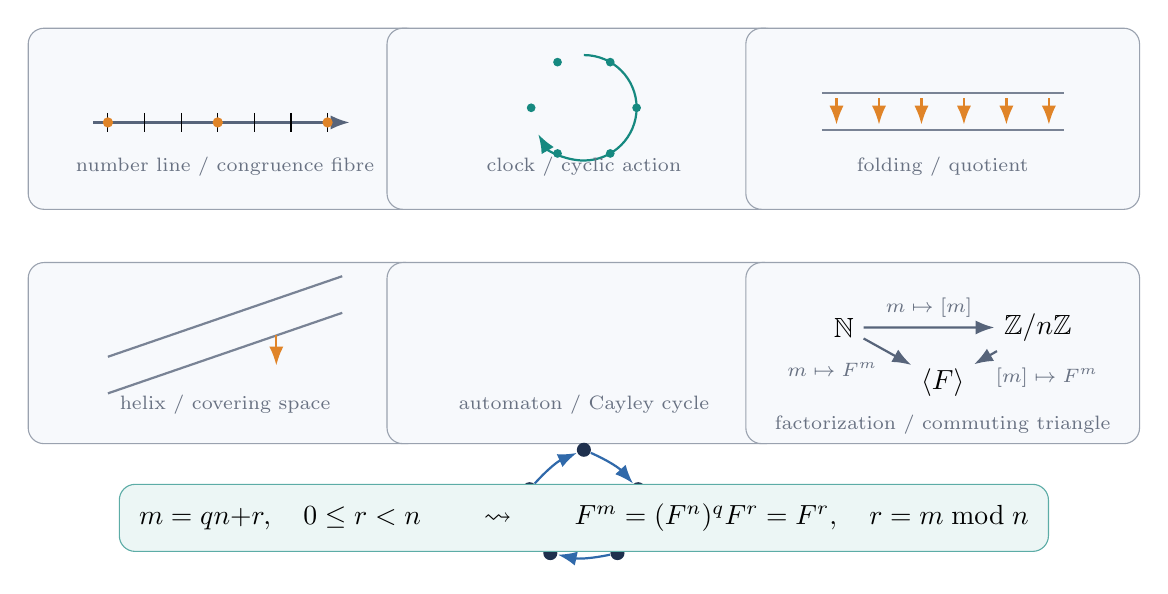
\begin{tikzpicture}[scale=.93]
  \node[soft,text width=4.4cm,minimum height=2.3cm] (line) at (-4.9,5.3) {};
  \draw[arr] (-6.7,5.25)--(-3.2,5.25);
  \foreach \x in {0,...,6}{\draw (-6.5+.5*\x,5.38)--(-6.5+.5*\x,5.12);}
  \foreach \x in {0,3,6}{\fill[orange] (-6.5+.5*\x,5.25) circle (2pt);}
  \node[lab] at (-4.9,4.65) {number line / congruence fibre};

  \node[soft,text width=4.4cm,minimum height=2.3cm] (clock) at (0,5.3) {};
  \foreach \a in {0,60,...,300}{\fill[teal] ($(0,5.45)+(\a:0.72)$) circle (1.7pt);}
  \draw[arr,teal] (0,5.45) +(90:.72) arc[start angle=90,end angle=-150,radius=.72];
  \node[lab] at (0,4.65) {clock / cyclic action};

  \node[soft,text width=4.4cm,minimum height=2.3cm] (fold) at (4.9,5.3) {};
  \draw[navy!60,thick] (3.25,5.65)--(6.55,5.65);
  \draw[navy!60,thick] (3.25,5.15)--(6.55,5.15);
  \foreach \x in {0,...,5}{\draw[arr,orange] (3.45+.58*\x,5.58)--(3.45+.58*\x,5.22);}
  \node[lab] at (4.9,4.65) {folding / quotient};

  \node[soft,text width=4.4cm,minimum height=2.3cm] at (-4.9,2.1) {};
  \draw[navy!60,thick] (-6.5,1.55)--(-3.3,2.65);
  \draw[navy!60,thick] (-6.5,2.05)--(-3.3,3.15);
  \draw[arr,orange] (-4.2,2.35)--(-4.2,1.93);
  \node[lab] at (-4.9,1.4) {helix / covering space};

  \node[soft,text width=4.4cm,minimum height=2.3cm] at (0,2.1) {};
  \foreach \i in {0,...,4}{\node[dot] (q\i) at (90-72*\i:.78) {};}
  \foreach \i in {0,...,4}{\pgfmathtruncatemacro{\j}{mod(\i+1,5)}\draw[arr,blue] (q\i) to[bend left=12] (q\j);}
  \node[lab] at (0,1.4) {automaton / Cayley cycle};

  \node[soft,text width=4.4cm,minimum height=2.3cm] at (4.9,2.1) {};
  \node (Z) at (3.55,2.45) {$\mathbb N$};
  \node (Q) at (6.2,2.45) {$\mathbb Z/n\mathbb Z$};
  \node (E) at (4.9,1.7) {$\langle F\rangle$};
  \draw[arr] (Z)--node[lab,above] {$m\mapsto[m]$}(Q);
  \draw[arr] (Z)--node[lab,below left] {$m\mapsto F^m$}(E);
  \draw[arr] (Q)--node[lab,below right] {$[m]\mapsto F^m$}(E);
  \node[lab] at (4.9,1.12) {factorization / commuting triangle};

  \node[eq,text width=11.3cm] at (0,-.15) {$m=qn+r,\quad 0\le r<n\qquad\rightsquigarrow\qquad F^m=(F^n)^qF^r=F^r,\quad r=m\bmod n$};
\end{tikzpicture}
\end{center}
\foot{Every plate below redraws this same normalization pattern.}
\newpage

% 2 — number lines
\head{1. Number Lines as Congruence Fibres}{$n=5$: vertical colour means equal Frobenius power}
\begin{center}
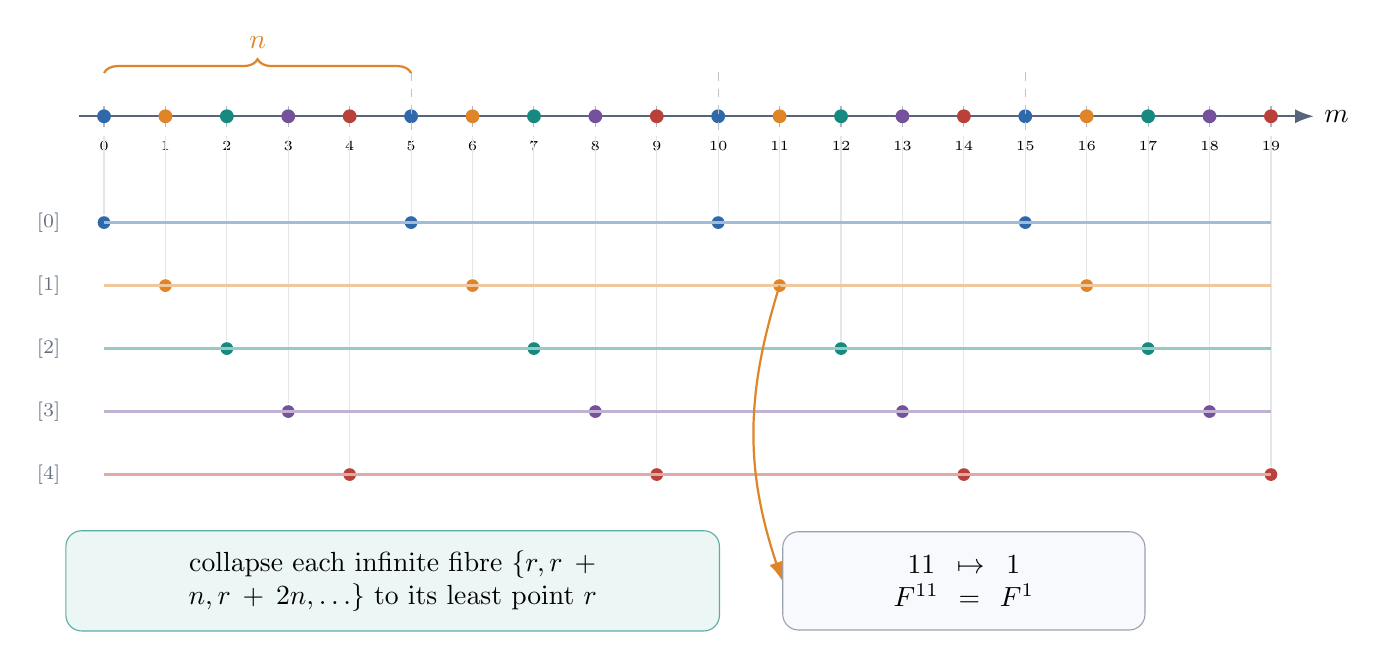
\begin{tikzpicture}[x=.78cm,y=1cm]
  \draw[arr] (-.4,5.8)--(19.7,5.8) node[right] {$m$};
  \foreach \x in {0,...,19}{
    \pgfmathtruncatemacro{\r}{mod(\x,5)}
    \draw[navy!35] (\x,5.93)--(\x,5.67);
    \node[below=2pt,font=\tiny] at (\x,5.67) {\x};
    \ifcase\r\fill[blue] (\x,5.8) circle (2.5pt);\or\fill[orange] (\x,5.8) circle (2.5pt);\or\fill[teal] (\x,5.8) circle (2.5pt);\or\fill[violet] (\x,5.8) circle (2.5pt);\or\fill[red] (\x,5.8) circle (2.5pt);\fi
  }
  \foreach \x in {5,10,15}{\draw[dashed,navy!30] (\x,5.2)--(\x,6.45);}
  \draw[decorate,decoration={brace,amplitude=5pt},orange,thick] (0,6.35)--(5,6.35) node[midway,above=5pt] {$n$};

  \node[lab,anchor=east] at (-.55,4.45) {$[0]$};
  \node[lab,anchor=east] at (-.55,3.65) {$[1]$};
  \node[lab,anchor=east] at (-.55,2.85) {$[2]$};
  \node[lab,anchor=east] at (-.55,2.05) {$[3]$};
  \node[lab,anchor=east] at (-.55,1.25) {$[4]$};
  \foreach \x in {0,...,19}{
    \pgfmathtruncatemacro{\r}{mod(\x,5)}
    \pgfmathsetmacro{\yy}{4.45-.8*\r}
    \ifcase\r\fill[blue] (\x,\yy) circle (2.3pt);\or\fill[orange] (\x,\yy) circle (2.3pt);\or\fill[teal] (\x,\yy) circle (2.3pt);\or\fill[violet] (\x,\yy) circle (2.3pt);\or\fill[red] (\x,\yy) circle (2.3pt);\fi
    \draw[navy!12] (\x,5.55)--(\x,\yy+.1);
  }
  \foreach \r/\c in {0/blue,1/orange,2/teal,3/violet,4/red}{\draw[\c!45,thick] (0,4.45-.8*\r)--(19,4.45-.8*\r);}

  \node[soft,text width=4cm] (eleven) at (14,-.1) {$11\mapsto 1$\\$F^{11}=F^1$};
  \draw[arr,orange,bend right=18] (11,3.65) to (eleven.west);
  \node[eq,text width=7.8cm] at (4.7,-.1) {collapse each infinite fibre $\{r,r+n,r+2n,\ldots\}$ to its least point $r$};
\end{tikzpicture}
\end{center}
\foot{$m\bmod n$ is a coordinate on the quotient, not merely a shorter exponent.}
\newpage

% 3 folding
\head{2. Folding the Infinite Strip}{Cut into periods; stack; project to the fundamental domain}
\begin{center}
\begin{tikzpicture}[x=.82cm,y=1cm]
  \foreach \row in {0,...,3}{
    \pgfmathsetmacro{\yy}{6.3-1.25*\row}
    \draw[navy!55,very thick] (0,\yy)--(5,\yy);
    \foreach \r in {0,...,5}{\draw[navy!35] (\r,\yy+.12)--(\r,\yy-.12);}
    \foreach \r in {0,...,4}{
      \pgfmathtruncatemacro{\m}{5*\row+\r}
      \node[font=\scriptsize] at (\r+.5,\yy+.28) {\m};
    }
    \node[lab,anchor=west] at (5.25,\yy) {$q=\row$};
  }
  \foreach \row in {1,...,3}{
    \pgfmathsetmacro{\ya}{6.3-1.25*\row}
    \foreach \r in {0,...,4}{\draw[arr,orange!70] (\r+.5,\ya+.18)--(\r+.5,6.08);}
  }
  \node[soft,rotate=90] at (-1.25,4.45) {discard quotient $q$};

  \draw[navy,very thick] (8,6.3)--(13,6.3);
  \foreach \r/\c in {0/blue,1/orange,2/teal,3/violet,4/red}{
    \fill[\c] (8.5+\r,6.3) circle (3pt);
    \node[above=5pt,font=\small] at (8.5+\r,6.3) {$\r$};
    \node[below=6pt,font=\scriptsize,text=\c] at (8.5+\r,6.3) {$F^{\r}$};
  }
  \node[lab] at (10.5,5.3) {fundamental domain $0\le r<n$};

  \node[soft,text width=12.2cm] at (6.4,2.25) {
    \begin{tikzpicture}[baseline]
      \node (m) at (0,0) {$m$};
      \node (qr) at (3,0) {$(q,r)$};
      \node (r) at (6,0) {$r=m\bmod n$};
      \node (fm) at (0,-1.25) {$F^m$};
      \node (prod) at (3,-1.25) {$(F^n)^qF^r$};
      \node (fr) at (6,-1.25) {$F^r$};
      \draw[arr] (m)--node[lab,above]{division}(qr);
      \draw[arr] (qr)--node[lab,above]{forget $q$}(r);
      \draw[arr] (m)--(fm);
      \draw[arr] (qr)--(prod);
      \draw[arr] (r)--(fr);
      \draw[arr] (fm)--node[lab,below]{unfold}(prod);
      \draw[arr] (prod)--node[lab,below]{$F^n=1$}(fr);
    \end{tikzpicture}
  };
\end{tikzpicture}
\end{center}
\foot{Euclidean division supplies the geometry: translation by $n$ changes the sheet, not the value.}
\newpage

% 4 clocks
\head{3. Frobenius Clocks}{Iteration moves one tick; the $n$th tick returns to the identity}
\begin{center}
\begin{tikzpicture}
  \foreach \cx/\nn/\col/\title in {-5/3/orange/$n=3$,0/5/teal/$n=5$,5/7/violet/$n=7$}{
    \node[font=\bfseries,text=navy] at (\cx,4.65) {\title};
    \draw[navy!25,thick] (\cx,3) circle (1.45);
    \foreach \i in {0,...,\nn}{
      \pgfmathsetmacro{\ang}{90-360*\i/\nn}
      \fill[\col] (\cx,3) +(\ang:1.45) circle (2.3pt);
    }
    \draw[-{Latex[length=2mm]},very thick,\col] (\cx,3)+(90:1.1) arc[start angle=90,end angle=-205,radius=1.1];
    \node[font=\scriptsize] at ($(\cx,3)+(90:1.82)$) {$0\equiv n$};
    \node[font=\small] at (\cx,3) {$F$};
  }

  \node[soft,text width=13.2cm] at (0,.15) {
    \begin{tikzpicture}[node distance=12mm]
      \node[dot,label=above:$F^0$] (a0) {};
      \node[dot,right=of a0,label=above:$F^1$] (a1) {};
      \node[dot,right=of a1,label=above:$F^2$] (a2) {};
      \node[right=of a2] (dots) {$\cdots$};
      \node[dot,right=of dots,label=above:$F^{n-1}$] (an) {};
      \draw[arr] (a0)--(a1);\draw[arr] (a1)--(a2);\draw[arr] (a2)--(dots);\draw[arr] (dots)--(an);
      \draw[arr,orange] (an) to[bend right=35] node[lab,below]{apply $F$; use $F^n=1$} (a0);
    \end{tikzpicture}
  };

  \node[eq,text width=11cm] at (0,-2.1) {$m$ steps on the infinite counter $\quad\longmapsto\quad$ the clock position $[m]_n$ $\quad\longmapsto\quad F^{[m]_n}$};
\end{tikzpicture}
\end{center}
\foot{The clock is the Cayley graph of the cyclic action generated by Frobenius.}
\newpage

% 5 covering / helix
\head{4. Helix, Cylinder, and Covering Map}{$\mathbb Z$ unwinds the cycle; modulo $n$ wraps it back}
\begin{center}
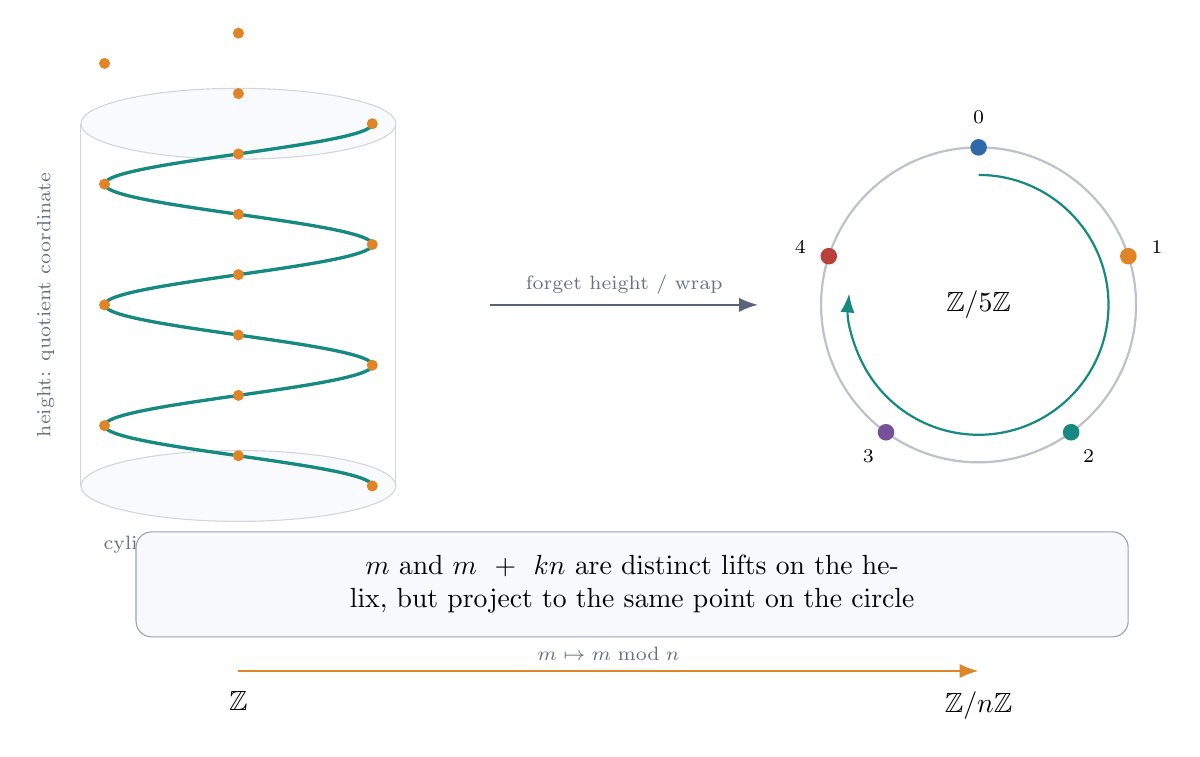
\begin{tikzpicture}[x=1cm,y=1cm]
  \draw[navy!20,fill=blue!3] (-5,1.1) ellipse (2 and .45);
  \draw[navy!20] (-7,1.1)--(-7,5.7) (-3,1.1)--(-3,5.7);
  \draw[navy!20,fill=blue!3] (-5,5.7) ellipse (2 and .45);
  \draw[very thick,teal,samples=180,domain=0:1080,smooth,variable=\t]
    plot ({-5+1.7*cos(\t)},{1.1+4.6*\t/1080});
  \foreach \k in {0,...,15}{
    \pgfmathsetmacro{\ang}{90*\k}
    \pgfmathsetmacro{\yy}{1.1+4.6*\k/12}
    \fill[orange] ({-5+1.7*cos(\ang)},\yy) circle (2pt);
  }
  \node[lab] at (-5,.35) {cylinder: residue coordinate};
  \node[lab,rotate=90] at (-7.45,3.4) {height: quotient coordinate};

  \draw[arr] (-1.8,3.4)--node[lab,above]{forget height / wrap} (1.6,3.4);

  \draw[navy!30,thick] (4.4,3.4) circle (2);
  \foreach \i/\c in {0/blue,1/orange,2/teal,3/violet,4/red}{
    \pgfmathsetmacro{\a}{90-72*\i}
    \fill[\c] ($(4.4,3.4)+(\a:2)$) circle (3pt);
    \node[font=\scriptsize] at ($(4.4,3.4)+(\a:2.38)$) {$\i$};
  }
  \draw[arr,teal] (4.4,3.4)+(90:1.65) arc[start angle=90,end angle=-185,radius=1.65];
  \node at (4.4,3.4) {$\mathbb Z/5\mathbb Z$};

  \node[soft,text width=12cm] at (0,-.15) {$m$ and $m+kn$ are distinct lifts on the helix, but project to the same point on the circle};
  \draw[arr,orange] (-5,-1.25)--node[lab,above] {$m\mapsto m\bmod n$} (4.4,-1.25);
  \node[below=4pt] at (-5,-1.25) {$\mathbb Z$};
  \node[below=4pt] at (4.4,-1.25) {$\mathbb Z/n\mathbb Z$};
\end{tikzpicture}
\end{center}
\foot{Normalization chooses the distinguished lift $0,1,\ldots,n-1$.}
\newpage

% 6 combinatorial
\head{5. Combinatorial Faces of the Same Quotient}{Beads, words, states, and orbits}
\begin{center}
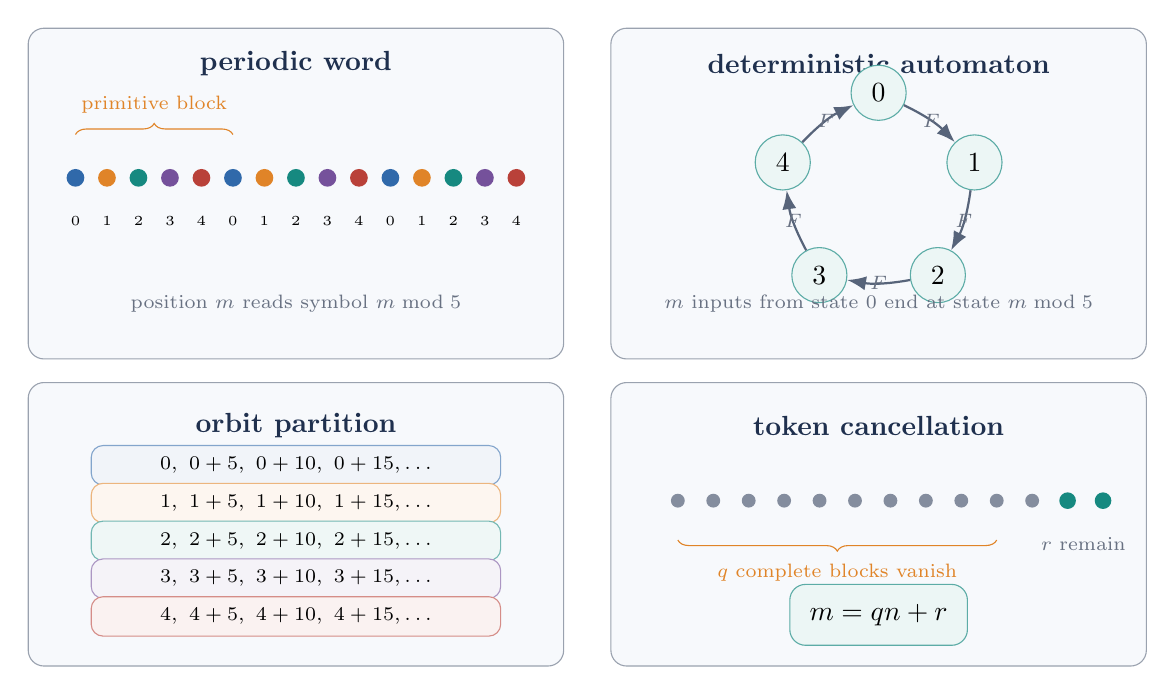
\begin{tikzpicture}
  \node[soft,text width=6.2cm,minimum height=4.2cm] at (-3.7,4.6) {};
  \node[font=\bfseries,text=navy] at (-3.7,6.25) {periodic word};
  \foreach \i in {0,...,14}{
    \pgfmathtruncatemacro{\r}{mod(\i,5)}
    \ifcase\r\def\cc{blue}\or\def\cc{orange}\or\def\cc{teal}\or\def\cc{violet}\or\def\cc{red}\fi
    \fill[\cc] (-6.5+.4*\i,4.8) circle (3.2pt);
    \node[font=\tiny] at (-6.5+.4*\i,4.25) {\r};
  }
  \draw[decorate,decoration={brace,amplitude=4pt},orange] (-6.5,5.35)--(-4.5,5.35) node[midway,above=4pt,font=\scriptsize] {primitive block};
  \node[lab] at (-3.7,3.2) {position $m$ reads symbol $m\bmod5$};

  \node[soft,text width=6.2cm,minimum height=4.2cm] at (3.7,4.6) {};
  \node[font=\bfseries,text=navy] at (3.7,6.25) {deterministic automaton};
  \foreach \i in {0,...,4}{\node[circle,draw=teal!70,fill=teal!8,minimum size=7mm] (s\i) at ($(3.7,4.6)+(90-72*\i:1.28)$) {$\i$};}
  \foreach \i in {0,...,4}{\pgfmathtruncatemacro{\j}{mod(\i+1,5)}\draw[arr] (s\i) to[bend left=10] node[lab] {$F$} (s\j);}
  \node[lab] at (3.7,3.2) {$m$ inputs from state $0$ end at state $m\bmod5$};

  \node[soft,text width=6.2cm,minimum height=3.6cm] at (-3.7,.4) {};
  \node[font=\bfseries,text=navy] at (-3.7,1.65) {orbit partition};
  \foreach \r/\c in {0/blue,1/orange,2/teal,3/violet,4/red}{
    \node[draw=\c!60,fill=\c!7,rounded corners=1.5mm,minimum width=5.2cm,minimum height=5mm,font=\scriptsize] at (-3.7,1.15-.48*\r) {$\r,\ \r+5,\ \r+10,\ \r+15,\ldots$};
  }

  \node[soft,text width=6.2cm,minimum height=3.6cm] at (3.7,.4) {};
  \node[font=\bfseries,text=navy] at (3.7,1.65) {token cancellation};
  \foreach \i in {0,...,11}{\fill[navy!55] (1.15+.45*\i,.7) circle (2.5pt);}
  \draw[decorate,decoration={brace,mirror,amplitude=4pt},orange] (1.15,.2)--(5.2,.2) node[midway,below=5pt,font=\scriptsize] {$q$ complete blocks vanish};
  \fill[teal] (6.1,.7) circle (3pt); \fill[teal] (6.55,.7) circle (3pt);
  \node[lab] at (6.3,.15) {$r$ remain};
  \node[eq] at (3.7,-.75) {$m=qn+r$};
\end{tikzpicture}
\end{center}
\foot{A complete block acts as $F^n=1$; only the incomplete tail remains.}
\newpage

% 7 geometric
\head{6. Geometric Normal Forms}{Translations, tessellations, and rotations}
\begin{center}
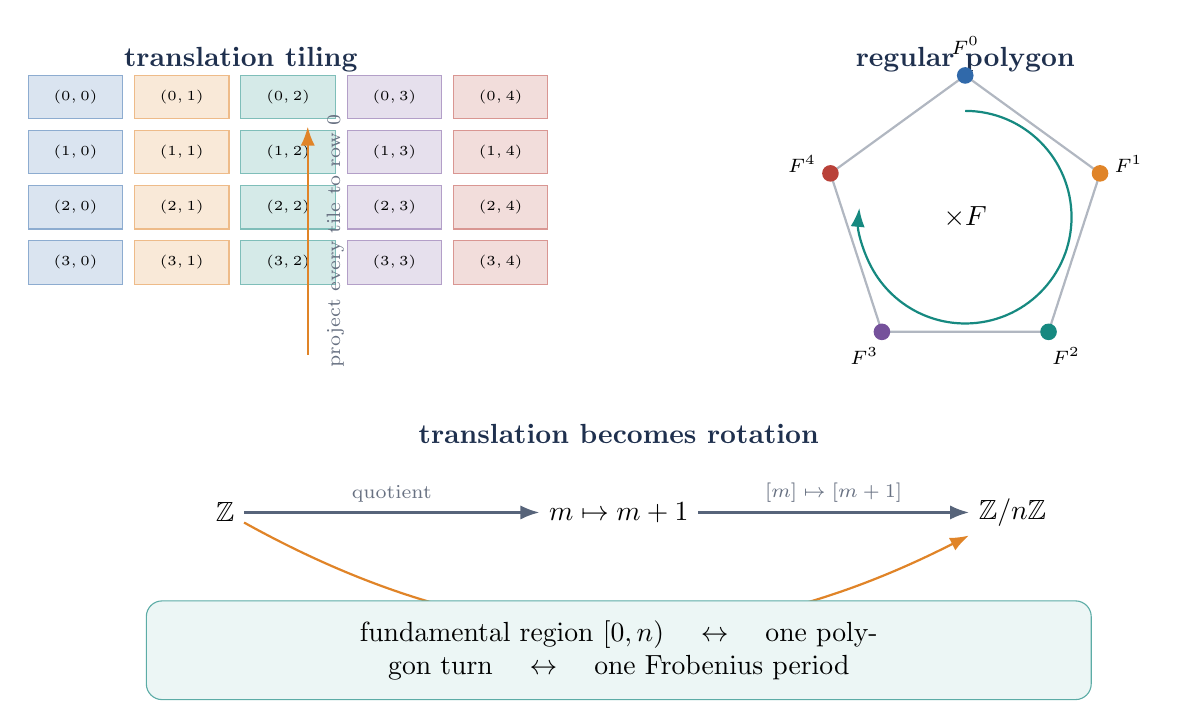
\begin{tikzpicture}
  \node[font=\bfseries,text=navy] at (-4.8,6.3) {translation tiling};
  \foreach \q in {0,...,3}{
    \foreach \r/\c in {0/blue,1/orange,2/teal,3/violet,4/red}{
      \fill[\c!18] (-7.5+1.35*\r,5.55-.7*\q) rectangle ++(1.2,.55);
      \draw[\c!55] (-7.5+1.35*\r,5.55-.7*\q) rectangle ++(1.2,.55);
      \node[font=\tiny] at (-6.9+1.35*\r,5.825-.7*\q) {$(\q,\r)$};
    }
  }
  \draw[arr,orange] (-3.95,2.55)--(-3.95,5.45);
  \node[lab,rotate=90] at (-3.6,4) {project every tile to row $0$};

  \node[font=\bfseries,text=navy] at (4.4,6.3) {regular polygon};
  \foreach \i in {0,...,4}{\coordinate (p\i) at ($(4.4,4.3)+(90-72*\i:1.8)$);}
  \draw[navy!35,thick] (p0)--(p1)--(p2)--(p3)--(p4)--cycle;
  \foreach \i/\c in {0/blue,1/orange,2/teal,3/violet,4/red}{\fill[\c] (p\i) circle (3pt);\node[font=\scriptsize] at ($(4.4,4.3)+(90-72*\i:2.18)$) {$F^{\i}$};}
  \draw[arr,teal] (4.4,4.3)+(90:1.35) arc[start angle=90,end angle=-185,radius=1.35];
  \node at (4.4,4.3) {$\times F$};

  \node[font=\bfseries,text=navy] at (0,1.55) {translation becomes rotation};
  \node (z) at (-5,.55) {$\mathbb Z$};
  \node (t) at (0,.55) {$m\mapsto m+1$};
  \node (c) at (5,.55) {$\mathbb Z/n\mathbb Z$};
  \draw[arr] (z)--node[lab,above]{quotient}(t);
  \draw[arr] (t)--node[lab,above]{$[m]\mapsto[m+1]$}(c);
  \draw[arr,orange] (z) to[bend right=28] node[lab,below]{$m\mapsto[m]$} (c);

  \node[eq,text width=11.5cm] at (0,-1.2) {fundamental region $[0,n)$ $\quad\leftrightarrow\quad$ one polygon turn $\quad\leftrightarrow\quad$ one Frobenius period};
\end{tikzpicture}
\end{center}
\foot{The modulo representative is the point inside a chosen fundamental region.}
\newpage

% 8 categories
\head{7. Commutative Diagrams}{The action factors uniquely through the quotient}
\begin{center}
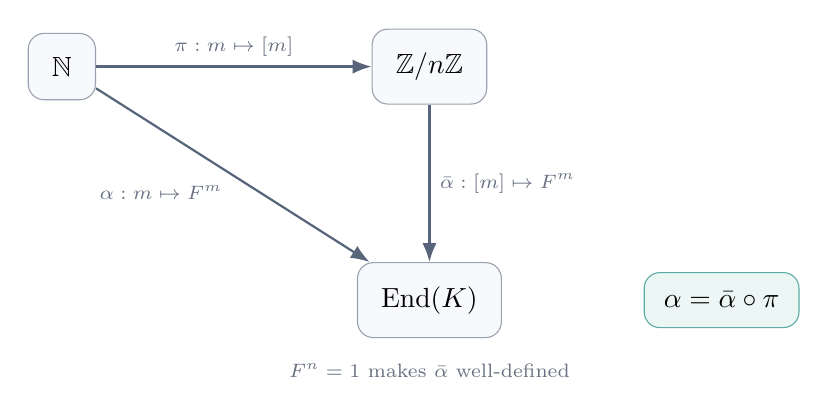
\begin{tikzpicture}[node distance=20mm and 35mm]
  \node[soft] (N) {$\mathbb N$};
  \node[soft,right=of N] (Q) {$\mathbb Z/n\mathbb Z$};
  \node[soft,below=of Q] (End) {$\operatorname{End}(K)$};
  \draw[arr] (N)--node[lab,above] {$\pi:m\mapsto[m]$}(Q);
  \draw[arr] (N)--node[lab,below left] {$\alpha:m\mapsto F^m$}(End);
  \draw[arr] (Q)--node[lab,right] {$\bar\alpha:[m]\mapsto F^m$}(End);
  \node[eq,right=18mm of End] {$\alpha=\bar\alpha\circ\pi$};
  \node[lab,below=2mm of End] {$F^n=1$ makes $\bar\alpha$ well-defined};
\end{tikzpicture}

\vspace{8mm}
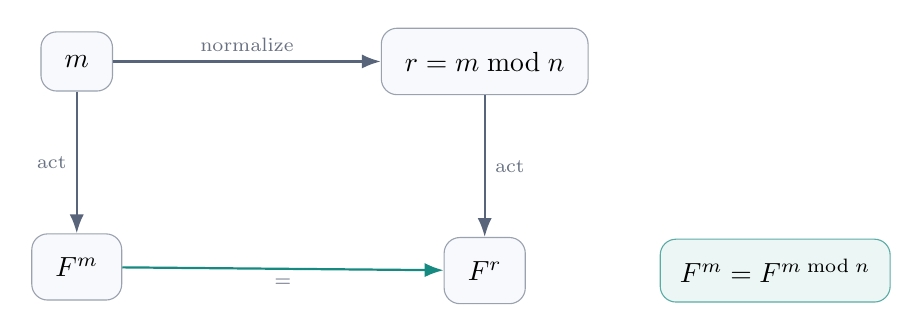
\begin{tikzpicture}[node distance=18mm and 34mm]
  \node[soft] (m) {$m$};
  \node[soft,right=of m] (r) {$r=m\bmod n$};
  \node[soft,below=of m] (Fm) {$F^m$};
  \node[soft,below=of r] (Fr) {$F^r$};
  \draw[arr] (m)--node[lab,above]{normalize}(r);
  \draw[arr] (m)--node[lab,left]{act}(Fm);
  \draw[arr] (r)--node[lab,right]{act}(Fr);
  \draw[arr,teal] (Fm)--node[lab,below]{$=$}(Fr);
  \node[eq,right=17mm of Fr] {$F^m=F^{m\bmod n}$};
\end{tikzpicture}

\vspace{8mm}
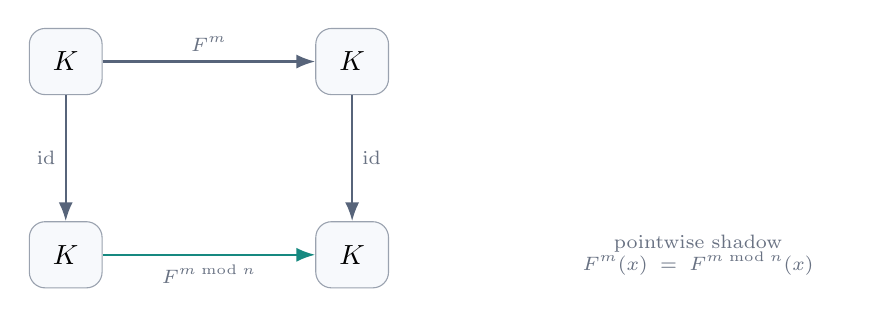
\begin{tikzpicture}[node distance=16mm and 27mm]
  \node[soft] (A) {$K$};
  \node[soft,right=of A] (B) {$K$};
  \node[soft,below=of A] (C) {$K$};
  \node[soft,below=of B] (D) {$K$};
  \draw[arr] (A)--node[lab,above]{$F^m$}(B);
  \draw[arr] (A)--node[lab,left]{$\mathrm{id}$}(C);
  \draw[arr] (B)--node[lab,right]{$\mathrm{id}$}(D);
  \draw[arr,teal] (C)--node[lab,below]{$F^{m\bmod n}$}(D);
  \node[lab,right=18mm of D,text width=4cm] {pointwise shadow\\$F^m(x)=F^{m\bmod n}(x)$};
\end{tikzpicture}
\end{center}
\foot{Categorically: a periodic monoid action descends along a quotient.}
\newpage

% 9 synthesis
\head{8. One Pattern, Nine Reading Directions}{Choose the picture that exposes the next proof step}
\begin{center}
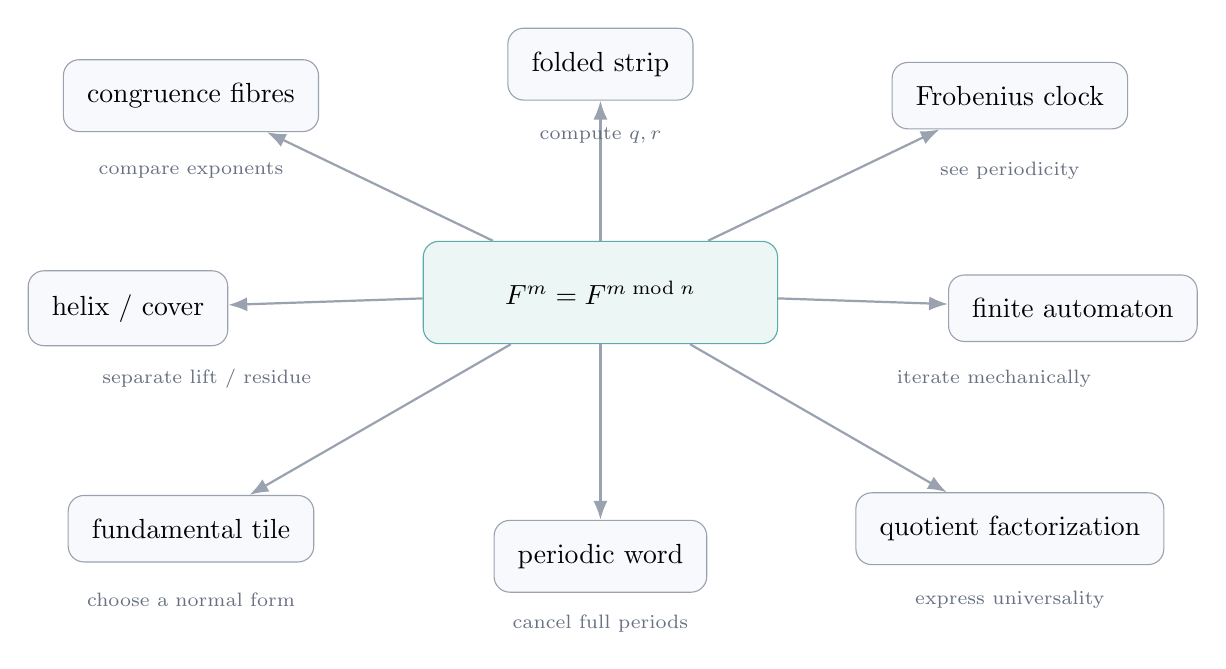
\begin{tikzpicture}
  \node[eq,minimum width=4.5cm,minimum height=1.3cm] (core) at (0,3.8) {$F^m=F^{m\bmod n}$};
  \node[soft] (line) at (-5.2,6.3) {congruence fibres};
  \node[soft] (fold) at (0,6.7) {folded strip};
  \node[soft] (clock) at (5.2,6.3) {Frobenius clock};
  \node[soft] (helix) at (-6,3.6) {helix / cover};
  \node[soft] (auto) at (6,3.6) {finite automaton};
  \node[soft] (tiles) at (-5.2,.8) {fundamental tile};
  \node[soft] (word) at (0,.45) {periodic word};
  \node[soft] (cat) at (5.2,.8) {quotient factorization};
  \foreach \n in {line,fold,clock,helix,auto,tiles,word,cat}{\draw[arr,navy!45] (core)--(\n);}

  \node[lab,text width=3.8cm] at (-5.2,5.35) {compare exponents};
  \node[lab,text width=3.8cm] at (0,5.8) {compute $q,r$};
  \node[lab,text width=3.8cm] at (5.2,5.35) {see periodicity};
  \node[lab,text width=3.8cm] at (-5,2.7) {separate lift / residue};
  \node[lab,text width=3.8cm] at (5,2.7) {iterate mechanically};
  \node[lab,text width=3.8cm] at (-5.2,-.1) {choose a normal form};
  \node[lab,text width=3.8cm] at (0,-.4) {cancel full periods};
  \node[lab,text width=3.8cm] at (5.2,-.1) {express universality};
\end{tikzpicture}
\end{center}
\vfill
\begin{center}
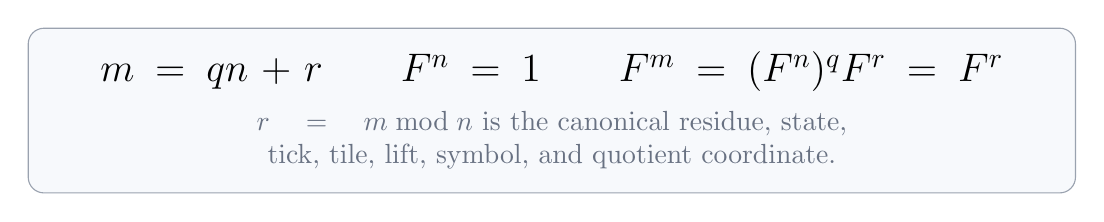
\begin{tikzpicture}
  \node[soft,text width=12.7cm,minimum height=1.9cm] {
    \Large $m=qn+r$\qquad $F^n=1$\qquad $F^m=(F^n)^qF^r=F^r$\\[2mm]
    \normalsize\color{muted}$r=m\bmod n$ is the canonical residue, state, tick, tile, lift, symbol, and quotient coordinate.};
\end{tikzpicture}
\end{center}
\foot{Visual companion to Section 1 of \code{FrobeniusPeriodicityAPIGuide.tex}.}

\end{document}
